\documentclass{article}
\usepackage[legalpaper, portrait, margin=0.5in]{geometry}
\usepackage {amsmath}
\usepackage {amssymb}
\usepackage {enumerate}
\usepackage{subcaption}
\usepackage{graphicx}
\usepackage{url}
\usepackage[breaklinks=true]{hyperref}
\usepackage{breakurl}

\title{CSC226 Assignment 2}
\author{Dryden Bryson}
\date{\today}

\begin{document}

\maketitle
\newpage
\section*{Introduction}
The $k$-source minimum cost path problem is a hybrid of the single source minimum cost path problem and the all-pairs minimum cost path problem, where instead of all or one source vertices, we pick an arbitrary value, $k$. We investigate two solutions to this problem, one involves using the Floyd-Warshall-Roy algorithm to find an all-pairs solution regardless of the value of $k$ and secondly we use Dijkstra's algorithm $k$ times.\\\\
Intuitively it might seem like using Dijkstra's algorithm $k$ times would be quicker since the FWR solution actually produces more data than neccesary and Dijkstra's is providing the minimum required information for the solution. It turns out that this intuition is actually false, in most cases using the FWR algorithm regardless of the value of $k$ is a more rapid solution to the $k$-source minimum cost path problem. It comes down to a mix of redundant operations occuring by repeating Dijkstra's repeatedly and the fundamental procedures of certain operations on CPU's. 

\subsection*{Methodology}
To compare the two afformentioned solutions to the $k$-source minimum cost path problem we will use experimental analysis. We have considered the following in the construction and execution of the experiment. 
\begin{itemize}
    \item \textbf{Programming Language and Hardware} C has been selected as the programming language of choice, due to it's relatively low level, which reduces abstraction overhead, minimizes unpredictability and has superior reproducability. The code was compiled using \texttt{gcc -O2}. The experiement was performed on the following hardware:
    \begin{itemize}
        \item i7-1360P processor (4 performance cores @ 5.00GHz, 8 efficiency cores @ 3.7GHz, 18Mb cache)
        \item 32Gb of 6000MT/s LPDDR5 Ram
        \item Windows 11 operating system, all other applications closed other then experiment, device in airplane mode and plugged in and performance options set to "best performance".
    \end{itemize}
    \item \textbf{Timing}, the windows "\texttt{QueryPerformanceCounter} is typically the best method to use to time-stamp events and measure small time intervals"\cite{microsoft_qpc} and was used to measure the execution time of exclusively the algorithm, algorithm initilization time was included. 
    \item \textbf{Domain of Experimentation} Every unique combination of the following parameters were tested and displayed as results for the experiment.
    \begin{itemize}
        \item Vertex counts from 25 to 500 in intervals of 25
        \item Graph densities (percentage of maximum possible edges given the number of vertices) from 25\%, 50\%, 75\% \& 100\%, 
        \item Values of $k$, which were given by the following percentage of total vertices in the graph, 1\%, 5\%, 10\%, 20\%, 30\%, ... 100\%
    \end{itemize}
    For each unique combination, 10 trials were run using different graphs and the median was selected from the 10 trials, an average coefficient of variation was calculated to be 6.74\% with smaller vertice counts experience more variation ($\sim$ 12\%) and large counts having less ($\sim$ 2\%) likely due to timer resolution limitations.
    \item \textbf{Graph Generation} The graphs were randomly generated by selecting a random origin vertex, destination vertex and edge weight, and repeatedly adding the generated edges ignoring duplicates and self loops until the target edge count was achieved. The random properties of the edges were generated using \texttt{rand()} which is generally not prefered but the likelyhood of affecting the graph structure in such a way that one algorithm is biased is very low. Source vertices were also selected using rand in a similar method to the edges, it falls victim to the same issues of \texttt{rand()} but again is very unlikely to have biased the experiment. 
    \item \textbf{Algorithm Implementation} To give both algorithms fair chance, they were implemented using different graph representations, adjacency linked list and adjacency matrix, for Dijkstra's and FWR respectively. Using only one implementation of a graph would have been unfair as either selection would biased one of the algorithms. Dijkstra's algorithm was implemented using a min-heap for maximum performance, this decision was made to ensure the most efficient version of both algorithms were used to simulate real world usage. 
\end{itemize}
\section*{Results}
By experimentation the following results were found:
\begin{figure}[h]
    \centering
    \begin{subfigure}{0.24\textwidth}
        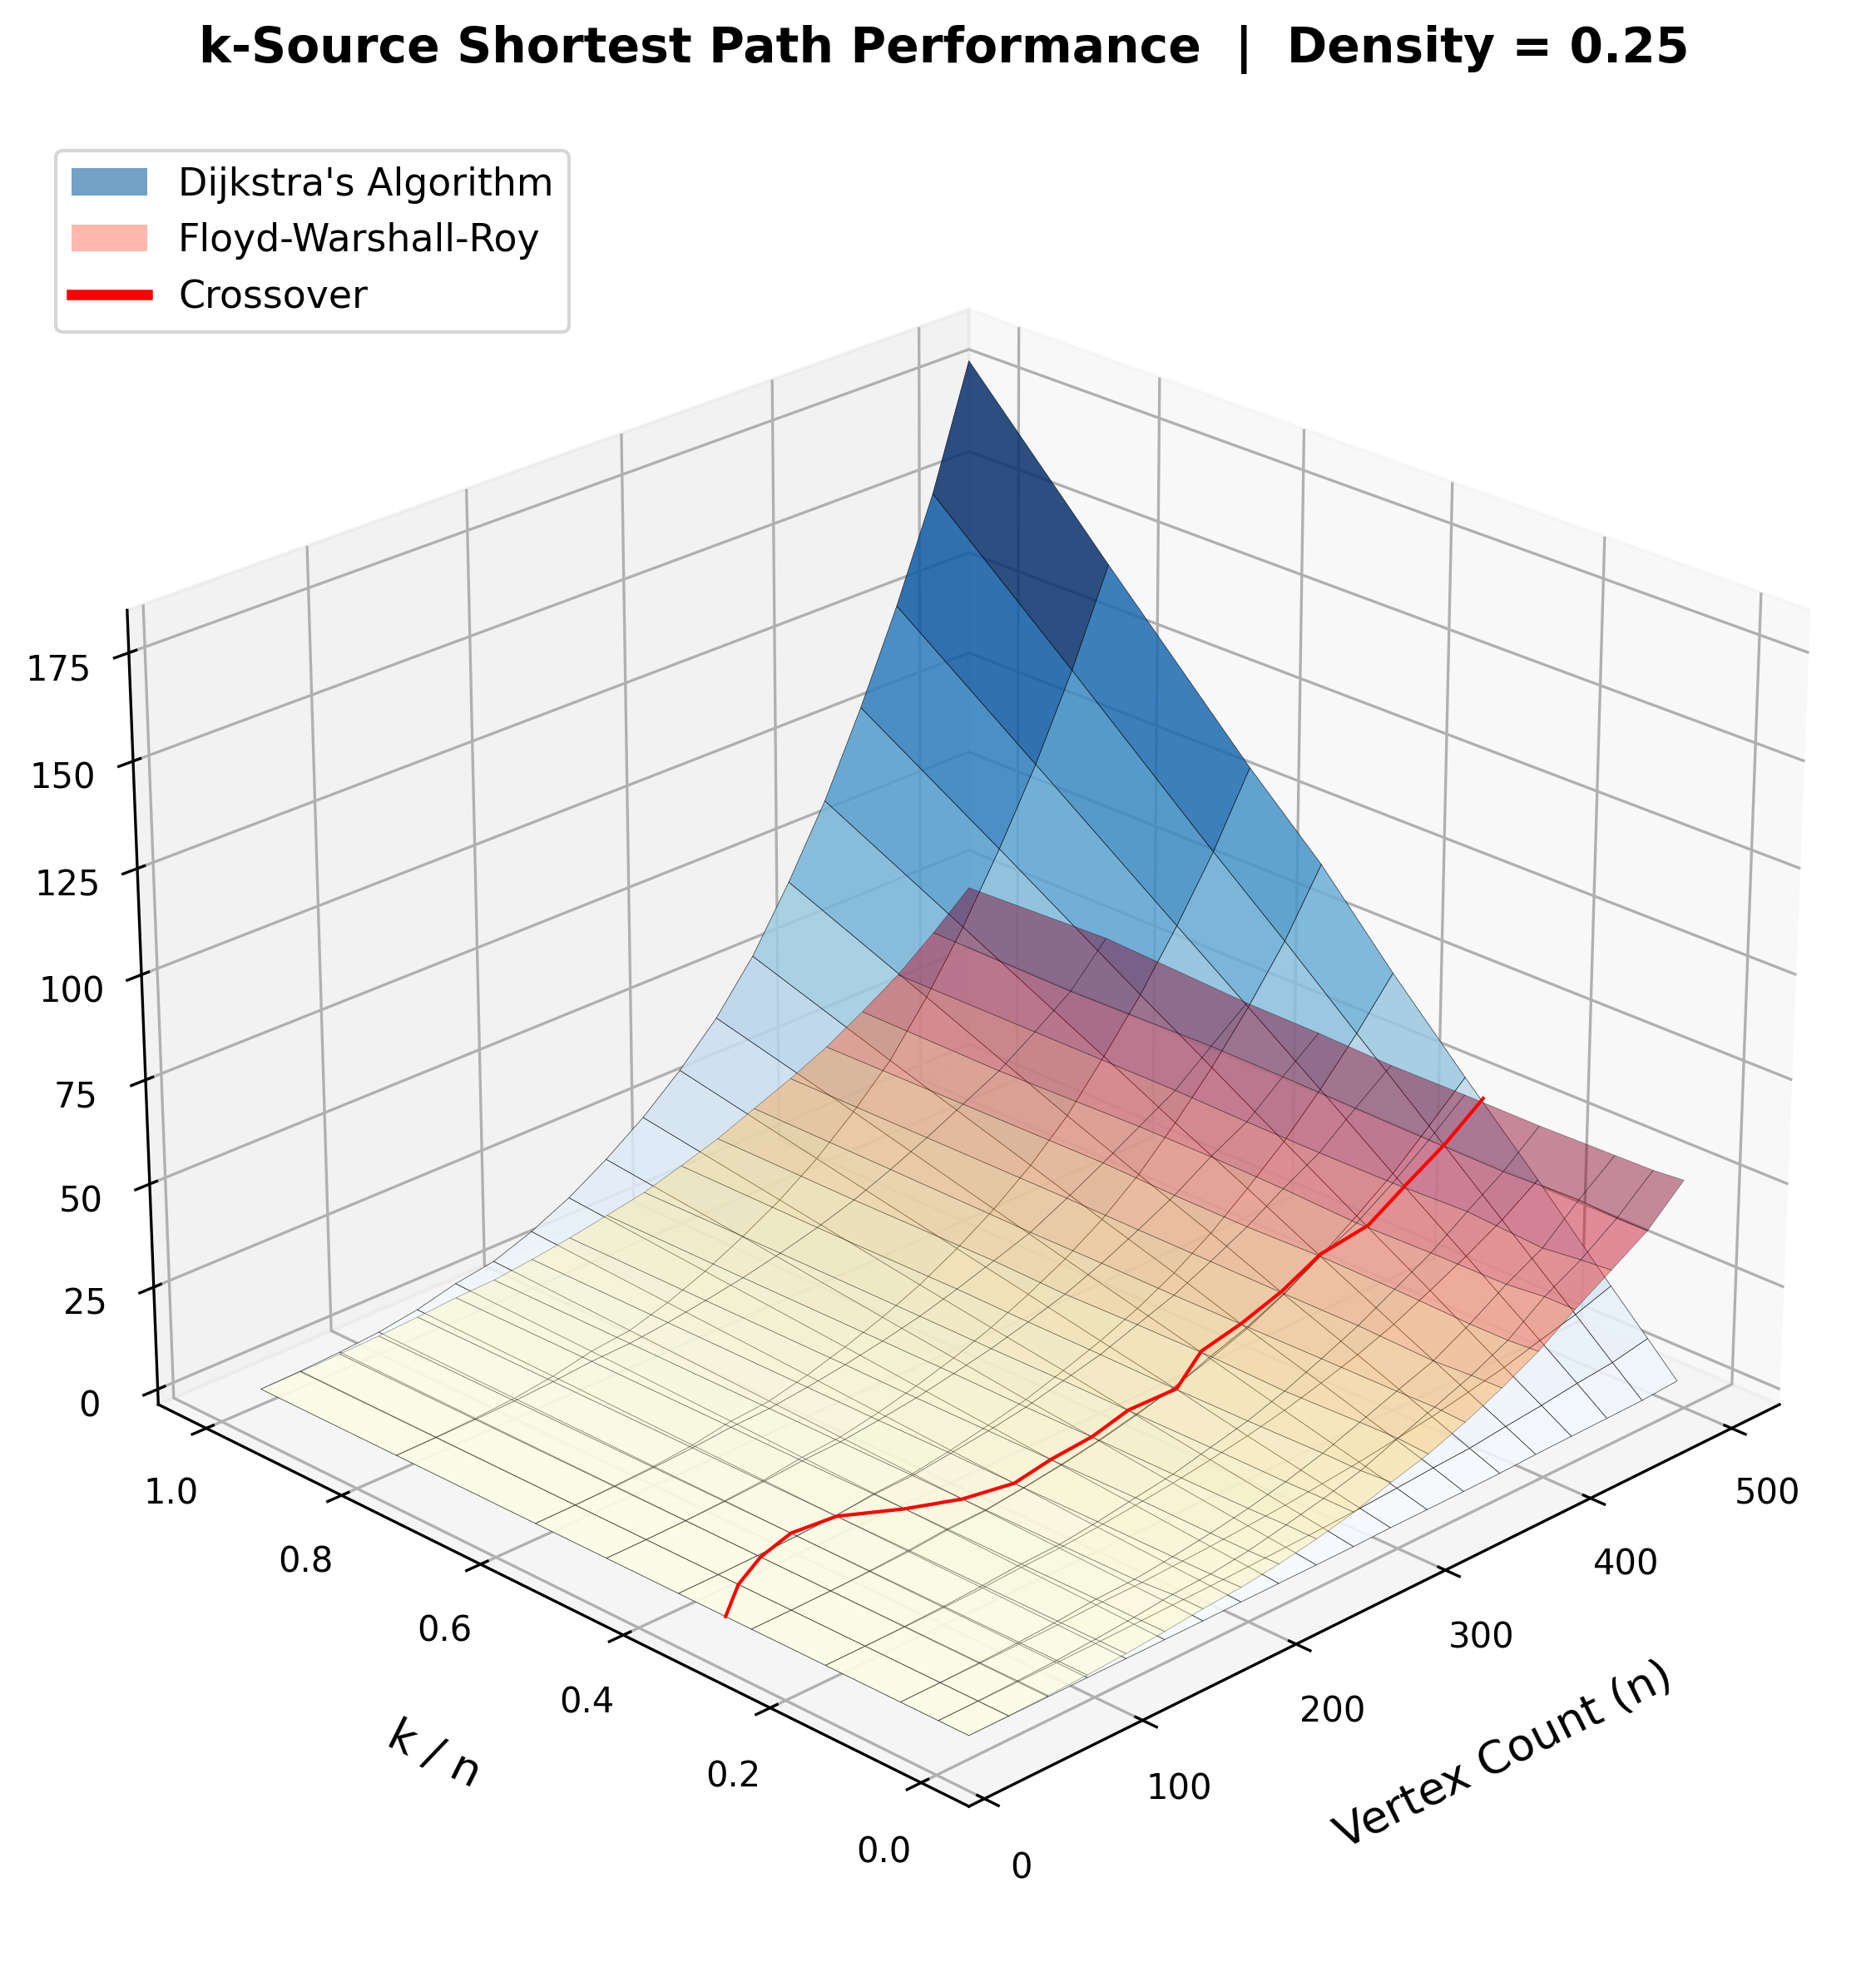
\includegraphics[width=\textwidth]{plot_density_0.25.png}
    \end{subfigure}
    \begin{subfigure}{0.24\textwidth}
        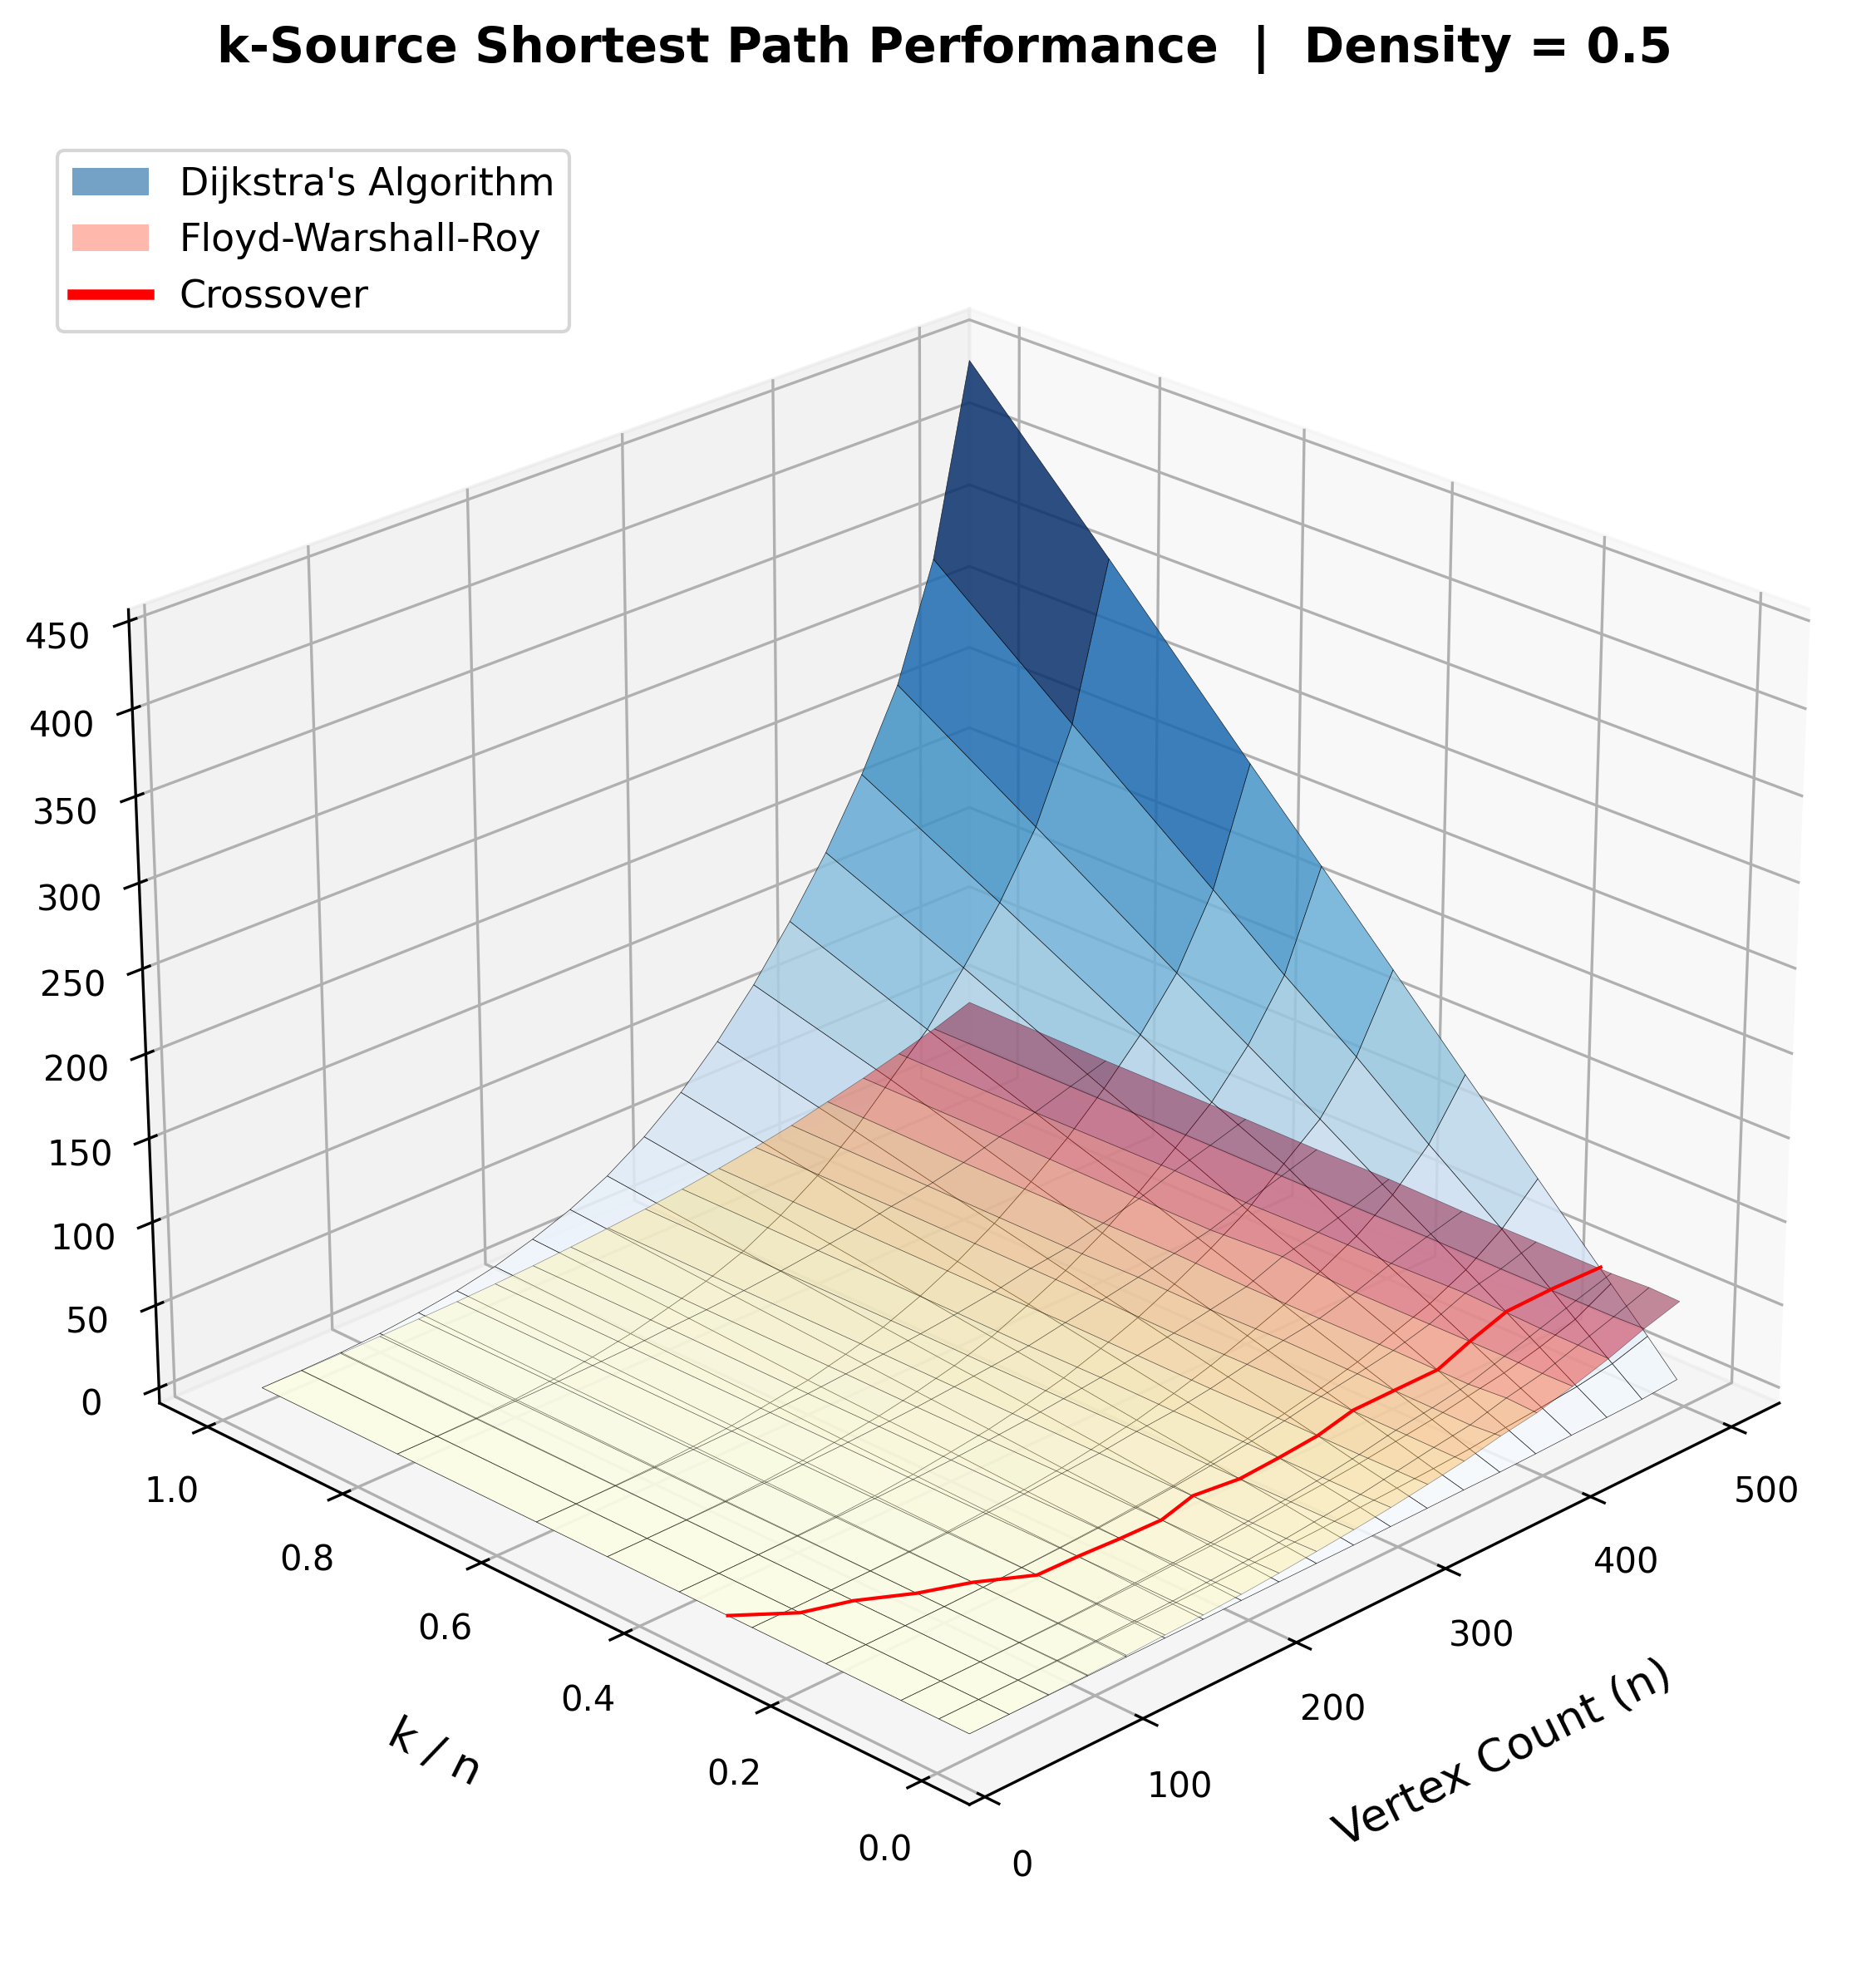
\includegraphics[width=\textwidth]{plot_density_0.5.png}
    \end{subfigure}
    \begin{subfigure}{0.24\textwidth}
        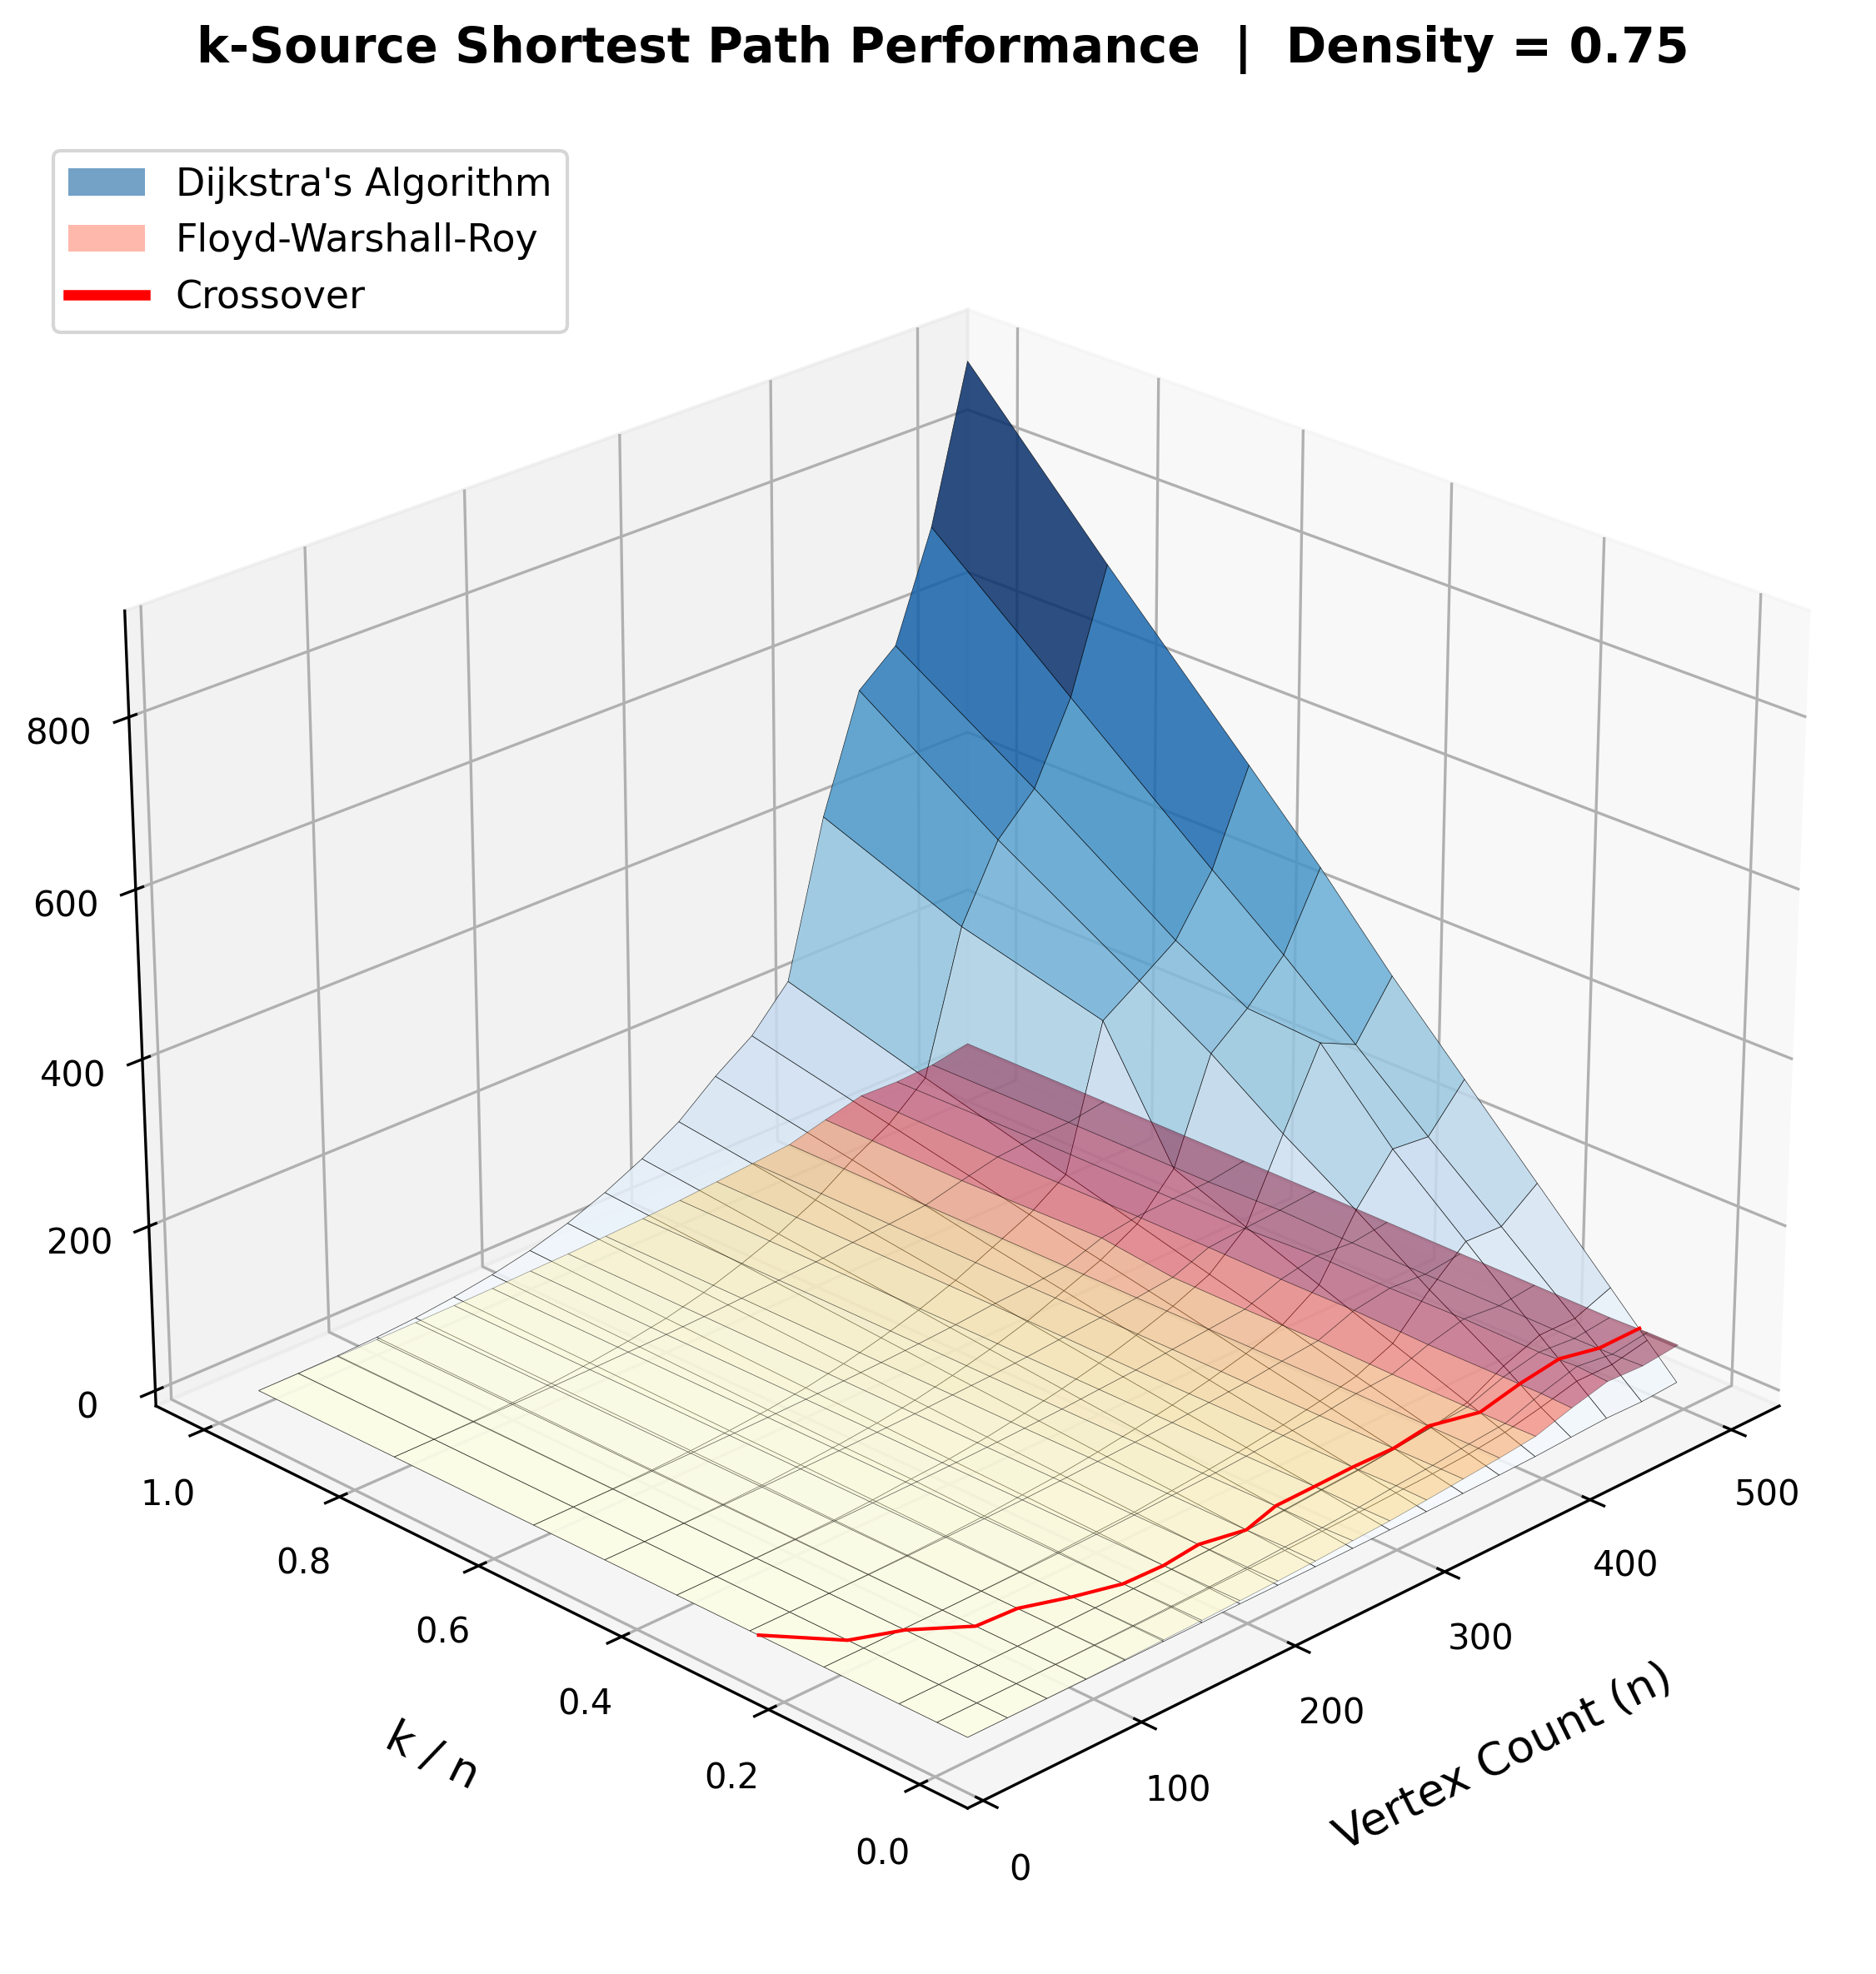
\includegraphics[width=\textwidth]{plot_density_0.75.png}
    \end{subfigure}
    \begin{subfigure}{0.24\textwidth}
        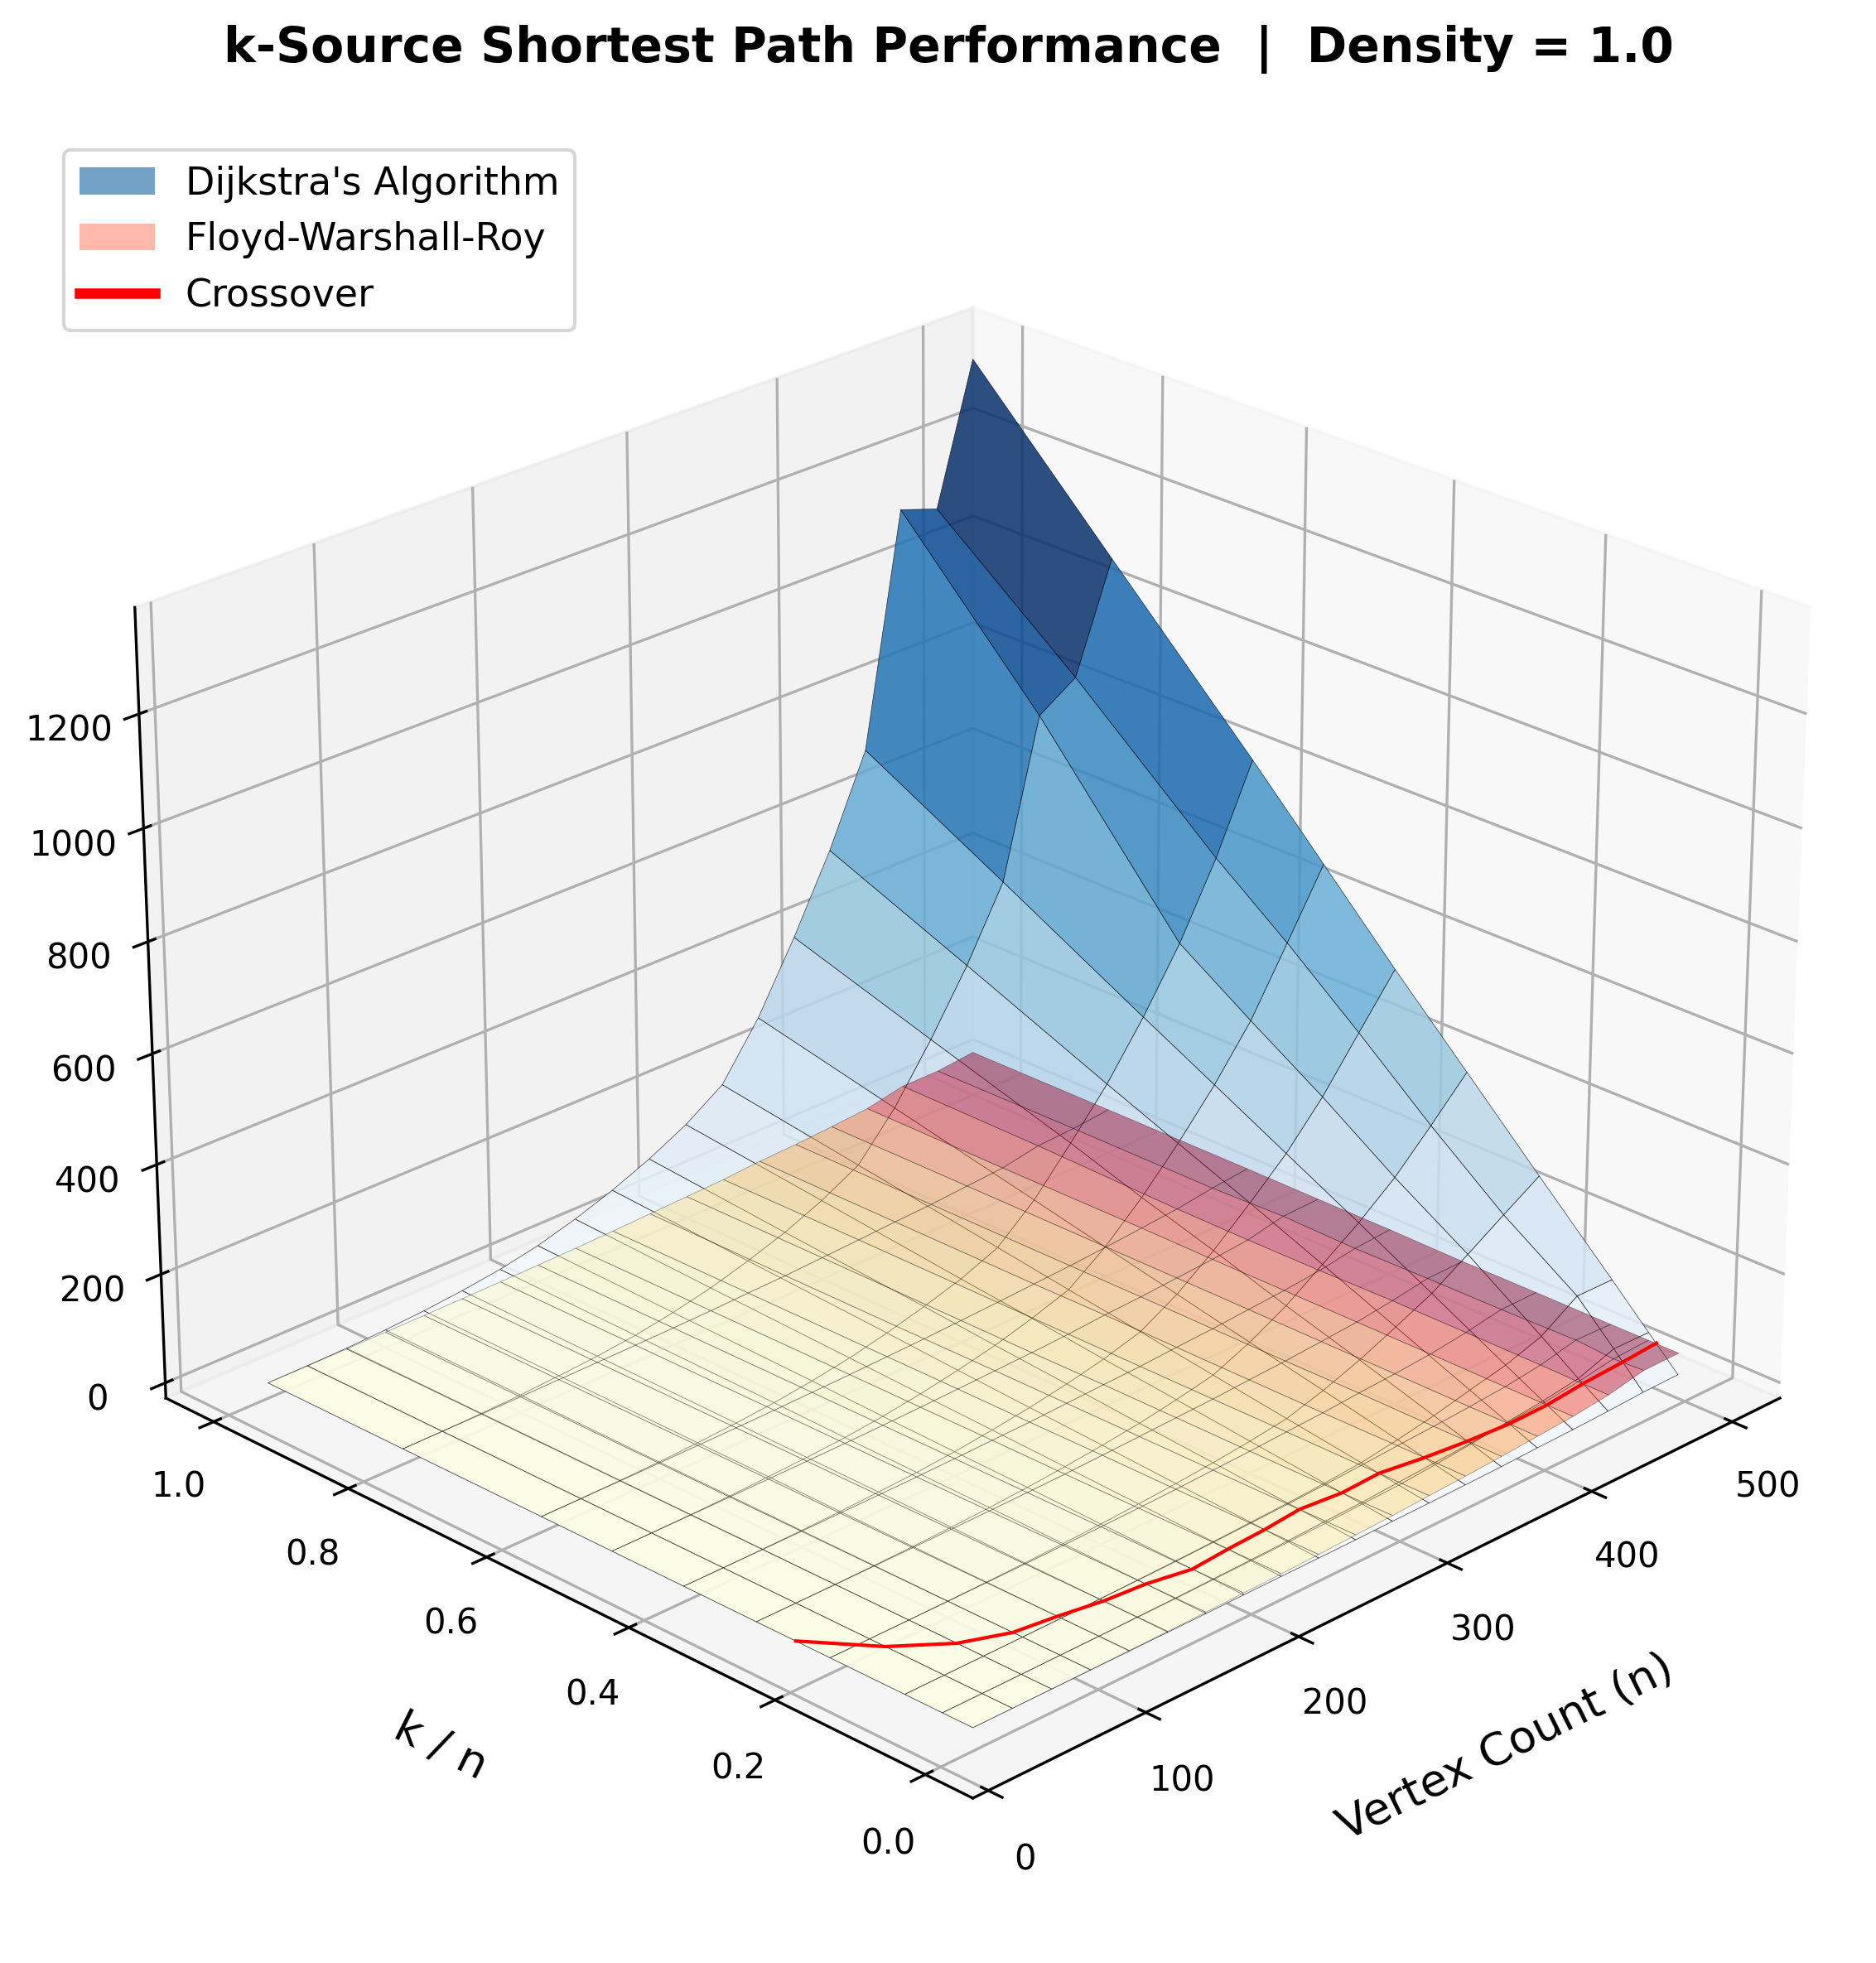
\includegraphics[width=\textwidth]{plot_density_1.0.png}
    \end{subfigure}
    \caption{k-Source Shortest Path Performance at densities 0.25, 0.50, 0.75, and 1.00}
    \label{fig:density_plots}
\end{figure}
The above figures show quite a clear picture substantiating the given conjecture, even for small values of $k$, the FWR algorithm is superior in terms of speed. Immediately we can see that for high $k$ values and high vertice counts, the time taken for Dijkstra's algorithm $k$ times absolutely explodes and absolutely does not compare to FWR. Now with a lower vertice count and smaller $k$ values they do become more comparable, but indicated by the red crossover line which indicates at which point FWR becomes quicker, the portion where FWR is slower is quite small\\\\
One notable point analyzing the crossoverline is that as the density increases, i.e more vertices per edge, the portion of experiments where FWR is slower becomes much smaller. This indicates that Dijkstra's algorithm suffers from very dense graphs and becomes slower which is logical, since the number of operations performed by the FWR algorithm is affected only by the number of vertices not edges. Given this when the graph is sparse, Djikstra's has better chance of keeping up with FWR.\\\\
Notably, the areas of the graph where we really begin to see a major seperation in the running time between the two is only after the vertice count exceeds $\sim$150 regardless of other parameters, this is possibly due to the small variances being hidden by the large peaks of Dijkstra's but even so difference would likely be less then $\sim$100ms. The most crucial part to analyze is that crossover line, since that directly substantiates or invalidates the conjecture, thus we have the following graph:
\begin{figure}[h]
    \centering
    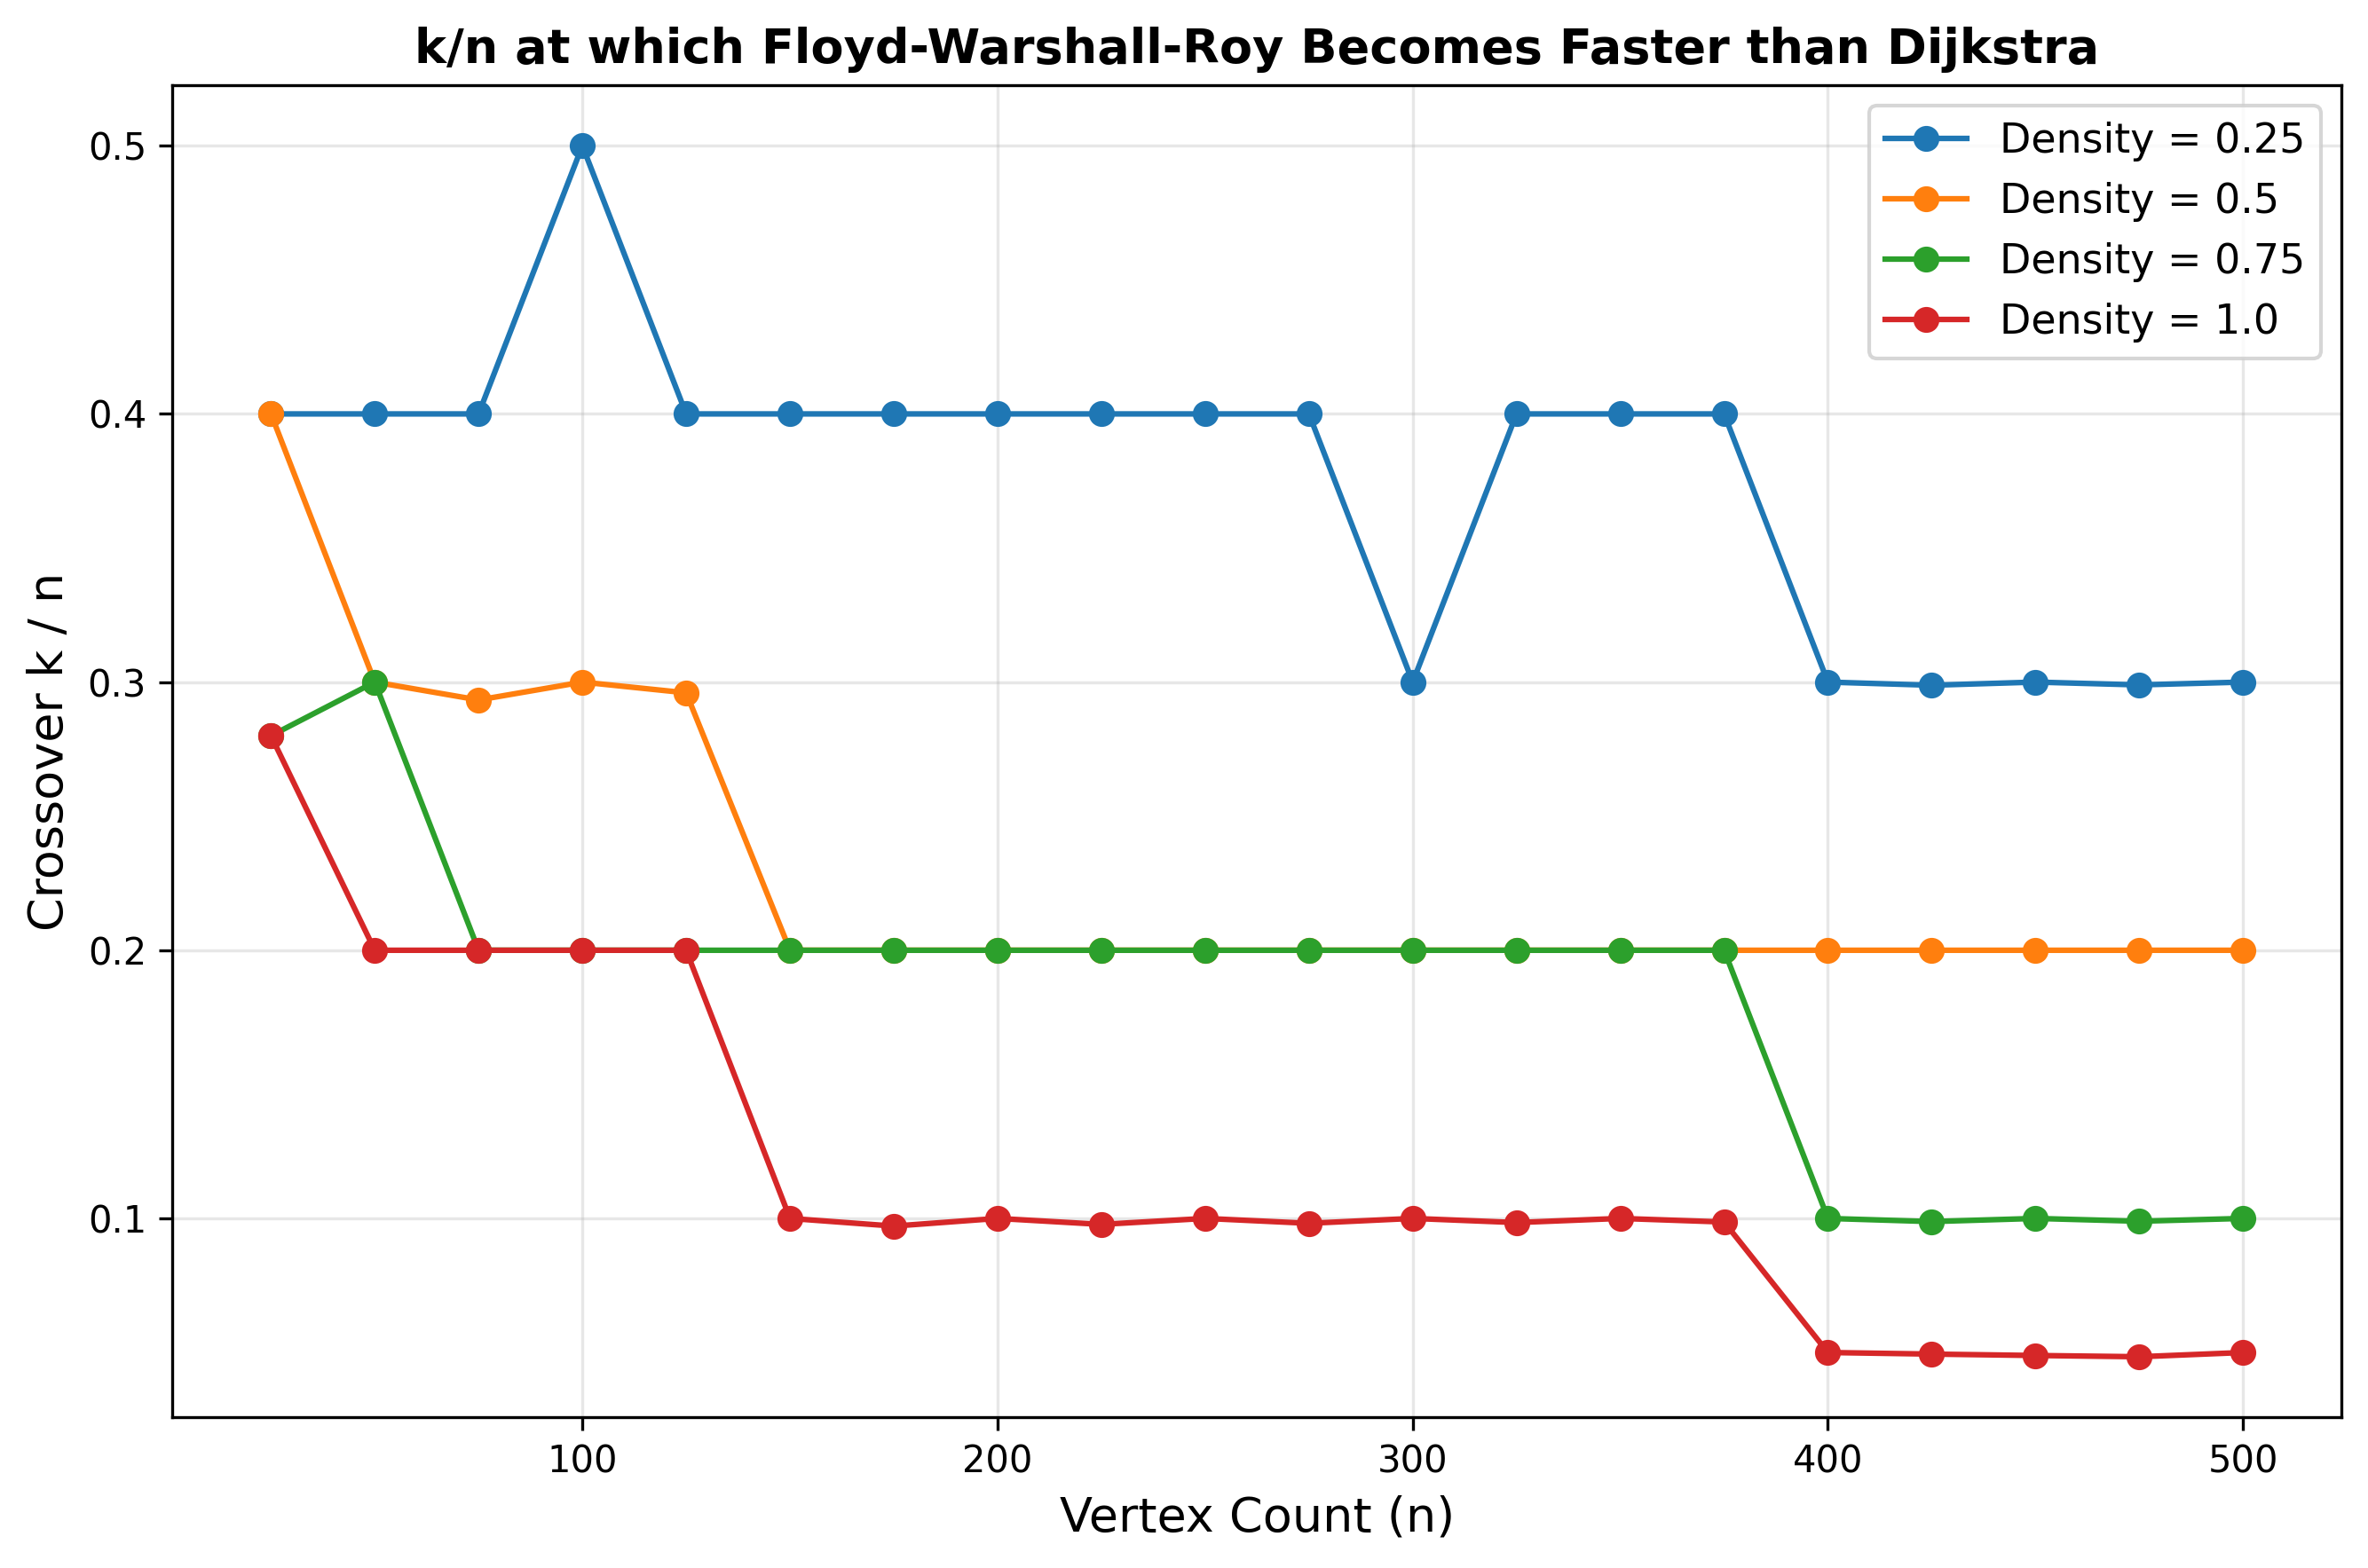
\includegraphics[width=0.75\textwidth]{plot_crossover.png}
    \caption{k/n at which Floyd-Warshall-Roy becomes faster than Dijkstra's algorithm across varying vertex counts and graph densities.}
    \label{fig:crossover}
\end{figure}
Again confirming what we determined previously from the 3D surface plots, as the vertex count increases, the value of $k$ at which FWR becomes faster decreases and as density increases that point also becomes lower. Since for values of $k$ we used fractions of the total number of vertices, we get the stepwise shape of the graph, but the true point would form a smoother line. But generally we can still see the trend. 

\section*{Conclusion}
In conclusion, we can say that the conjecture is justified and substantiated by the results of our experimentation, for some small values of $k$ running Djikstra's $k$ times can be faster but the portion of the cases where that is true are relatively small. On average FWR is faster then Dijkstra's once $k$ exceeds approximately 23\% of the vertex count with the threshold decreasing to approximately 16\% for larger graphs and incrasing to 30\% for smaller graphs. FWR is also faster when the graphs are very dense, i.e contianing a large amount of edges relative to the number of vertices.\\\\
This demonstrates that asymptotic complexity is not sufficient alone to determine the practical efficiency of algorithms given that FWR has a larger asymptotic run time, factors beyond what can be measured by counting operations often play a larger role then what is shown with asymptotic notation. \\\\
The reasons why FWR is faster are thus hard to determine but some educated guesses can be made: 
\begin{itemize}
    \item \textbf{Simpler Code} while this seems irrelevant, code compilers are much better at optimizing simple code such as the triple loop in FWR, comparitevly the underyling heap structure used in Dijkstra's is far more complicated and less likely to be optimized, other factors like the branching occuring in Dijkstra's and the use of pointers can also lead to issues like cache misses and pointer chasing. While optimization could have been disabled to provide a more "fair" chance to Dijkstra's, to simulate real world performance this was not done. 
    \item \textbf{Redundant Work} running Dijkstra's multiple times exposes it to multiple potential areas of redundant work, most likely to cause issues is the initialization and freeing of the heap, at $k/n=1$ that is 500 heap initializations and free's. Aswell Dijkstra's may be traversing certain paths repeatedly. 
\end{itemize}  
There are surely more reasons beyond this but it is more so speculation without more in depth profiling, but regardless the conclusion is the same and we can certainly say that the given conjecture is true. 

\newpage
\begin{thebibliography}{9}

\bibitem{microsoft_qpc}
Microsoft Corporation.
\textit{Acquiring High-Resolution Time Stamps}.
Windows App Development Documentation.
\href{https://learn.microsoft.com/en-us/windows/win32/sysinfo/acquiring-high-resolution-time-stamps}{Microsoft Docs: Acquiring High-Resolution Time Stamps}

\bibitem{dijkstra_video1}
Bird, B.
\textit{Algorithm Science (Summer 2025) - 35 - Minimum Cost Paths II}.
YouTube, 2019.
\href{https://www.youtube.com/watch?v=ANZpc0zhc9Q}{YouTube: Algorithm Science (Summer 2025) - 35 - Minimum Cost Paths II}

\bibitem{dijkstra_video2}
Bird, B.
\textit{Dijkstra Algorithm}.
YouTube.
\href{https://www.youtube.com/watch?v=BejY7uiUhEs}{YouTube: Dijkstra Algorithm}

\bibitem{thealgorithms_dijkstra}
TheAlgorithms.
\textit{dijkstra.c}.
GitHub, \textit{C} repository.
\href{https://github.com/TheAlgorithms/C/blob/master/greedy_approach/dijkstra.c}{GitHub: TheAlgorithms/C dijkstra.c}

\bibitem{thealgorithms_fwr}
TheAlgorithms.
\textit{floyd\_warshall.c}.
GitHub, \textit{C} repository.
\href{https://github.com/TheAlgorithms/C/blob/master/data_structures/graphs/floyd_warshall.c}{GitHub: TheAlgorithms/C floyd\_warshall.c}

\bibitem{thealgorithms_heap}
TheAlgorithms.
\textit{min\_heap.c}.
GitHub, \textit{C} repository.
\href{https://github.com/TheAlgorithms/C/blob/master/data_structures/heap/min_heap.c}{GitHub: TheAlgorithms/C min\_heap.c}

\bibitem{dt2450_dijkstra}
dt2450.
\textit{dijkstra\_directed.c}.
GitHub.
\href{https://github.com/dt2450/Dijkstras-Algorithm/blob/master/dijkstra_directed.c}{GitHub: dt2450/Dijkstras-Algorithm dijkstra\_directed.c}

\bibitem{baeldung_heap}
Baeldung.
\textit{Decrease-Key Operation in Min-Heaps}.
Baeldung on Computer Science.
\href{https://www.baeldung.com/cs/min-heaps-decrease-key}{Baeldung: Decrease-Key Operation in Min-Heaps}

\end{thebibliography}
\end{document}
